\documentclass[11pt,a4paper]{article}

% -------------------------------------------------------------
%   Packages
% -------------------------------------------------------------
\usepackage[utf8]{inputenc}
\usepackage[T1]{fontenc}
\usepackage{lmodern}
\usepackage{geometry}
\usepackage{graphicx}
\usepackage{caption}
\usepackage{subcaption}
\usepackage{listings}
\usepackage{xcolor}
\usepackage{courier}
 
\lstset{
	basicstyle=\ttfamily\small,
	keywordstyle=\color{blue}\bfseries,
	commentstyle=\color{gray}\itshape,
	stringstyle=\color{orange},
	breaklines=true,
	showstringspaces=false,
	frame=single,
	captionpos=b,
	language=R
}
\usepackage{booktabs}
\usepackage{siunitx}
\usepackage{amsmath,amsfonts,amssymb}
\usepackage{hyperref}
\usepackage{float}
\usepackage{cleveref}
\usepackage{enumitem}
\usepackage[gen]{eurosym}  % For \EUR{} symbol

% -------------------------------------------------------------
%   Page layout
% -------------------------------------------------------------
\geometry{margin=1in}
\setlength{\parskip}{0.6em}
\setlength{\parindent}{0pt}

% -------------------------------------------------------------
%   Title data
% -------------------------------------------------------------
\title{Performance of Trading Strategies for Hedging Options\\[0.5em]\large R Project 2025}
\author{Marcus-Adrian Piso (i6314615) \\ Yves Seuren (i6384237)\\ Denny Tran (i6398792)\\ Cas Brands (i6394851)}
\date{\today}

\begin{document}
	\maketitle
	
	\begin{abstract}
		This project studies and compares three hedging strategies for a six-month call on a European stock \textit{BrightFuture} using a lognormal price model. 
		We use a Monte Carlo engine (100{,}000 paths, daily rebalancing) to simulate the three strategies: no hedge, \textit{stop-loss} --- purchase 100 shares only when the underlying exceeds the strike, and a Black--Scholes delta hedge. 
		We compute the option premium \( P_0 \) for each strategy, to find the 99\% profit premiums in part b), then analyse the resulting \textit{P\&L} (profit and loss) distribution. ß
		Indifference prices are derived based on a utility function of Constant Absolute Risk Aversion (\textit{CARA}) ußtility. 
		Per our results, the unhedged trader's bank should charge \( \approx \EUR{3400} \), with the stop-loss trader being quoted \( \approx \EUR{1600} \), and the delta-hedger \( \approx \EUR{360} \).
		
		From the perspective of a risk-averse trader, the indifference prices we solve for in section d) push the strategies more further apart; while the unhedged bank raises the quote considerably, the delta-hedger’s premium rises only marginally. 
		The stop-loss trader once again ends up in the middle, but still presents with a long tail of losses – rare, but significant – once the price slips back under the strike price. 
		In the end, our simulations turn formulas into ready to present numbers, that show exactly how much protection each hedge will buy.
	\end{abstract}
	
	\tableofcontents
	\newpage
	% =============================================================
	\section{Introduction}
	\subsection{Motivation}
	Generally, selling options is very appealing for an experienced trader because the seller receives an immediate premium. However, like with all financial derivatives, risk can be substantial --- if the underlying stock’s price rises sharply, so do the losses. Traders manage this risk by employing hedging methods, of which there are three in our project: a \textit{stop-loss hedge}, where the trader buys/sells the stock only if its price crosses the strike; the \textit{delta hedge}, which continuously adjusts a hedge based on the price movements of that stock; or \textit{no hedge} --- the trader accepts full exposure.
	
	At this point, probabilistic modelling plays a very important role. It’s challenging to evaluate how effective these hedges are, since future stock/asset prices behave randomly and under uncertainty. Therefore, we implement a Monte Carlo simulation, simulating a very large number (in our case 100{,}000) of possible future stock-price scenarios, letting us analyze and compare the risks of every hedging strategy.
	
	\subsection{Objectives and Methodology}
The main goal of the project is to use R and especially the Monte Carlo method to meticulously analyze each strategy. Specifically, we implemented the following methods:

We generate \(100{,}000\) daily price paths and assume a lognormal model for stock prices, with an expected yearly return of \(10\%\) and a \(20\%\) standard deviation. To ensure we get realistic daily price movements, we generate random shocks from a normal distribution, then calculate the stock price at each step (through cumulative exponentiation) --- this allows us to track how each of the strategies performs over the full six months.

We calculate \(P_0\) --- the premium that each trader’s bank should charge to guarantee a \(99\%\) profit (\(1\%\) loss probability), to build a clear safety measure for each strategy. We accomplish this by running all the simulations, calculating the final profit or loss for each strategy, and then taking the \(1\%\) quantile of the resulting distributions.

Next, we analyse the resulting \textit{P\&L} (profit and loss) distributions using histograms to visualize the full range of outcomes. This way we can specifically notice the tail-risk, the aforementioned rare but significant losses that each strategy carries, to gain an intuitive understanding of the frequency of extreme outcomes.

For the next point, we define a \textit{CARA} (Constant Absolute Risk Aversion) utility function that captures different levels of risk aversion. We supplement this with numerical root-finding (the \texttt{uniroot} function in R) to solve for the \textit{indifference premium}, at which the trader is equally well-off (in terms of expected utility) if they buy or sell the option. We can clearly extract how sensitive option prices are to risk preferences by repeating this calculation over an arbitrary range of risk aversion, specifically
\[
a \in \{0.001,\ 0.002,\ 0.005,\ 0.01,\ 0.03,\ 0.05\}.
\]
We initially experimented with more and higher levels, but for values like \(0.05\), the expected utility function becomes nearly flat, making the root difficult to bracket and leading to unrealistic results. Our range covers the industry standard for analyses of low to even moderate risk aversion for a decision-maker.

Finally, we evaluate the \textit{conditional risk probability} from the stop-loss strategy, more specifically examining the probability of loss if the stock price temporarily falls below a certain barrier before expiry (which we set at \(\euro90\), a 10\% draw-down). We check all the simulated paths to see how often the price falls below this at any given point, and then check which of these paths lead to a loss at the time of expiry. A high conditional probability means that the stop-loss frequently misses the moment --- the trader sells the stock near the bottom, cashing out right before the market rallies past the strike. The trader is forced to deliver \(100\) shares at the time of expiry with no long position, freezing the payoff for the holder --- in this case we notice that the stop-loss hedge is effective for steady movements but easily prone to heavy losses under high volatility. In contrast, if only a handful of paths go below the strike, the stop-loss rule does its job correctly. A low result suggests that the barrier is placed well and the trader can effectively ``shed'' risk during down-trends without missing the rally.
	
	\subsection{Structure of the Report}
	
	We have organized the report to move logically from modelling to insights and discussion. In the next section we \textit{``set the stage''}, formulating the lognormal process we are using for the share price of BrightFuture and declaring all the parameters (see Table~\ref{tab:params}). Then, in Section 3 we present our findings from the simulation as follows:
	\begin{itemize}
		\item Quantify the simple probability that the call finishes ITM (in-the-money)
		\item Derive the \( P_0 \) profit premium for each of the three banks
		\item Visualize and comment on the resulting profit-and-loss-distributions
		\item Compute and repot CARA indifference prices across the interval we defined earlier
		\item Evaluate the conditional failure probability once the barrier has been reached for the stop-loss strategy.
	\end{itemize}
	
	Section 4 follows, where we discuss and pull all the results together. We compare the efficiency of the hedges, the quotes themselves (or capital requirements) + tail risk, highlight the trade-offs between each. We conclude the report by discussing the main points for a trading desk and contouring points where future work could sharpen our analysis even further. Appendix A contains additional code we use for our that is not included in the original code for compatibility (we call \texttt{hrbrthemes} and \texttt{patchwork}, the former requiring install through \texttt{remotes}, essentially it would be too much clutter in the main code).
	
\subsection{Log-Normal Stock-Price Dynamics}

We model the evolution of the share price according to the solution \( S_t \) of a geometric Brownian motion (GBM) from the Black--Scholes option pricing model. So over one trading day step \( \Delta t = \frac{1}{365} \), the price changes as follows:
\[
S_{t+\Delta t} = S_t \,\exp\!\left[(\mu - \tfrac{1}{2}\sigma^{2})\,\Delta t
+ \sigma\sqrt{\Delta t}\,Z_{t+\Delta t}\right],
\qquad Z_{t+\Delta t} \sim \mathcal{N}(0,1)\ \text{i.i.d.}
\]

\( \mu \) is the mean continuously-compounded return; which is given as \( \mu = 10\% \) p.a. \\
\( \sigma \) is the volatility, which is given at \( 20\% \) p.a. \\
The shocks \( Z_{t+\Delta t} \) are independent standard normal variables, which verify \( \mathbb{P}(A \cap B) = \mathbb{P}(A)\mathbb{P}(B) \).

The lognormal distribution arises from the distribution of the logarithm of \( S_t \). To keep the error low/negligible, we generate 100{,}000 price paths for the Monte Carlo simulation, each of them with 183 daily computed steps to match the time frame of the option (half a year). Moreover, by the Law of Large Numbers, the averages from the simulation converge quickly; with the \( N \) we choose, the sampling error is going to be under 1\%.

\subsection{Contract Parameters}

All the other values are fixed and declared in the table that follows. Risk-free rate: all cash balances grow at this rate \( \Rightarrow\; \text{\euro}1 \) in \( t \) years becomes \( e^{rt} \). Barrier for the stop-loss hedge: when the price falls to \( \text{\euro}90 \), we essentially “flag” it to isolate the weaknesses in this strategy later on. These parameters are constant throughout the analysis and we declare them together clearly to keep the environment and code clean and free of clutter.
	
	\begin{table}[H]
		\centering
		\caption{Baseline parameter set}
		\label{tab:params}
		\begin{tabular}{@{}llc@{}}
			\toprule
			Symbol & Meaning & Value \\
			\midrule
			$S_0$ & Initial stock price & \EUR{100} \\
			$K$   & Strike price        & \EUR{110} \\
			$T$   & Time to maturity    & 183 days \\
			$r$   & Risk‑free rate      & \SI{3}{\percent~p.a.} \\
			$\mu$ & Expected return     & \SI{10}{\percent~p.a.} \\
			$\sigma$ & Volatility       & \SI{20}{\percent~p.a.} \\
			\bottomrule
		\end{tabular}
	\end{table}
	
	% =============================================================
	% =============================================================
	\section{Results}
	\subsection{Probability Call Ends In‑the‑Money}
	Based on our Monte Carlo simulation, we find the following estimate for the probability that the call option ends in-the-money: \[
	\hat{p}_{\text{ITM}} = 0.34778
	\]
	Therefore we can infer that in $\approx$ 34.8\% of the cases, the stock exceelds the strike - the option will expire with a positive payoff, giving it intrinsic value at time of maturity.
	\subsection{Premiums Ensuring 99\,\% Profit}
	To make sure the previous assumption of 99\% profit holds, we compute the amount that the trader's bank must charge upfront as premium under each of the hedging strategies. This is the 1\% quantile of the Profit and Loss distribution. We have the following results:

\begin{table}[H]
	\centering
	\caption{Required premium $P_0$ to ensure 99\% profitability}
	\label{tab:premiums}
	\begin{tabular}{@{}lc@{}}
		\toprule
		Strategy & Premium (\EUR{}) \\
		\midrule
		No-hedge (Alice)    & 3421.26 \\
		Stop-loss (Bradley) & 1592.08 \\
		Delta-hedge (Claire) & 363.98 \\
		\bottomrule
	\end{tabular}
\end{table}
	Due to the high probability of substantial losses, the no-hedge strategy needs to be quoted the highest premium. The other two lower the risk and therefore the premium, with the delta-hedge strategy approaching closely the fair price of the call as it seems to correctly predict losses and safely ''withdraw''.
\subsection{Profit \& Loss Distributions}

\begin{figure}[H]
	\centering
	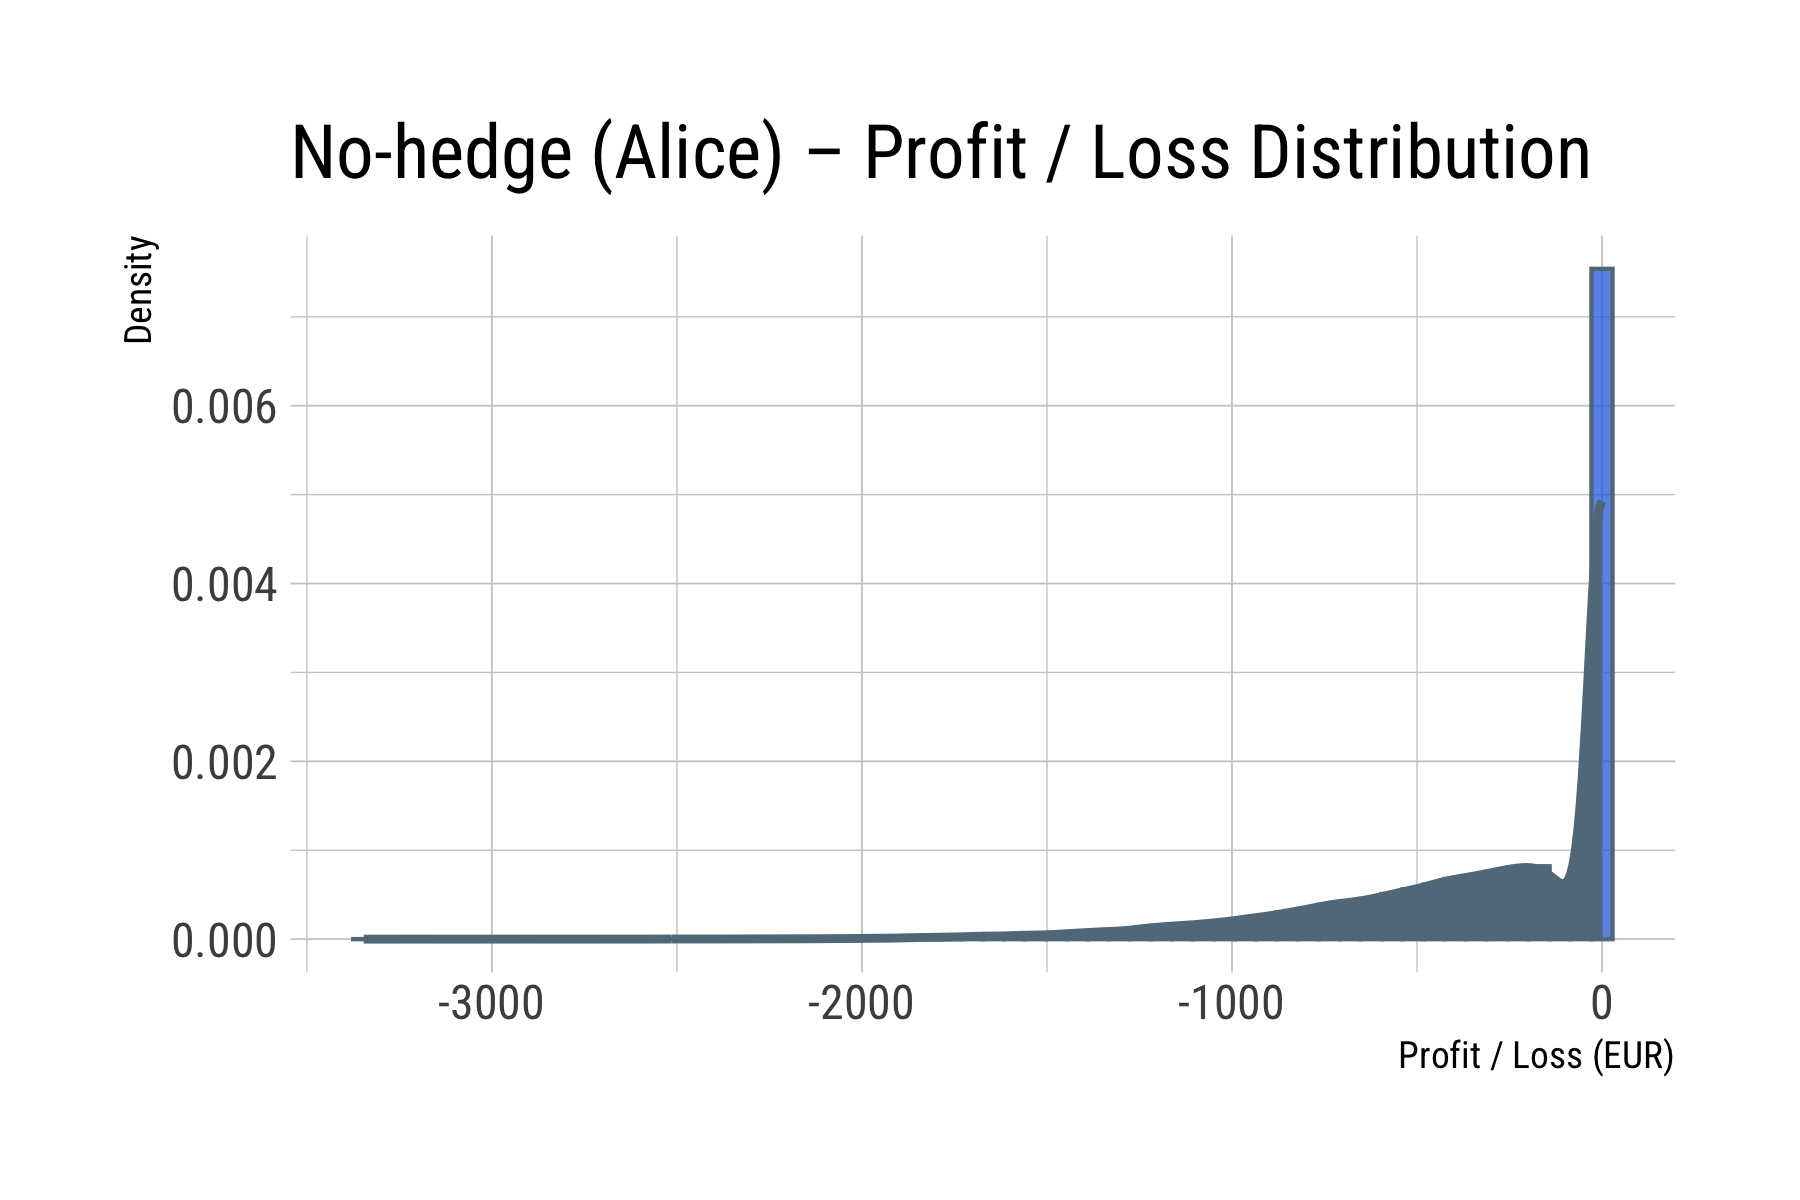
\includegraphics[width=0.85\linewidth]{figures/pnl_alice.png}
	\caption{Profit/Loss distribution — No-hedge (Alice)}
	\label{fig:pnl_alice}
\end{figure}

We start with Alice — who does not hedge at all. Her P\&L distribution \([\,\text{Figure~\ref{fig:pnl_alice}}\,]\) is skewed to the right, indicating that the bulk of the outcomes is close to the quoted premium, which is quite intuitive; the lack of any hedging means that the option ends out-of-the-money and is therefore worthless. The main ``issue'' with this strategy is that in the rare cases the option finishes well in-the-money, the losses can become massive as she must pay the entire intrinsic value. In a real trade scenario, such an event on the tail end would invalidate many small gains on the other end.

\begin{figure}[H]
	\centering
	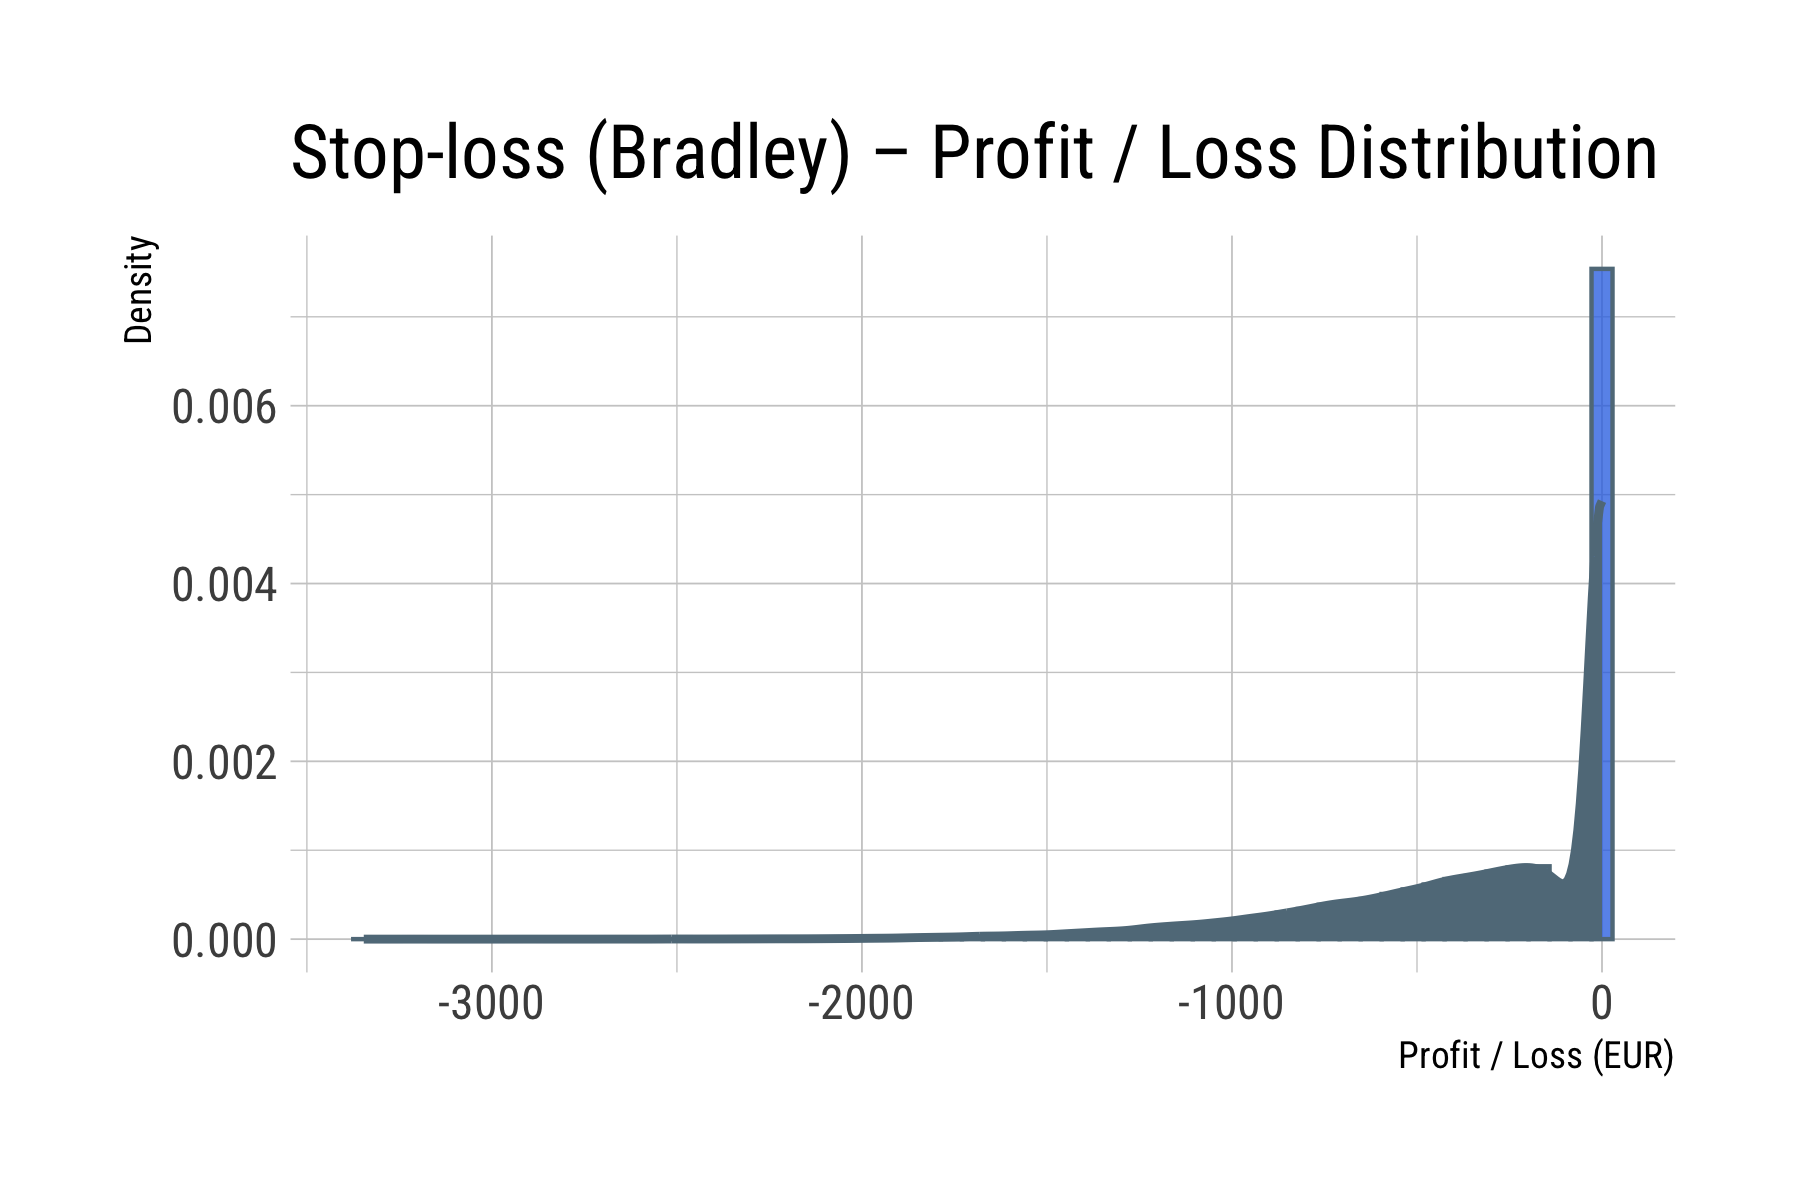
\includegraphics[width=0.85\linewidth]{figures/pnl_bradley.png}
	\caption{Profit/Loss distribution — Stop-loss(Bradley)}
	\label{fig:pnl_bradley}
\end{figure}

For Bradley, the stop-loss trader, his distribution in \([\,\text{Figure~\ref{fig:pnl_bradley}}\,]\) shows that the left tail is smaller but not negligible. We understand that when the stock rises steadily, the hedge works — his long position appreciates as the liability of the option does. In this case, the problem is when the price oscillates between gains and losses. A short plunge in price below €90 followed by a rise would force Bradley flat because of his stop-loss before he takes any profits.

\begin{figure}[H]
	\centering
	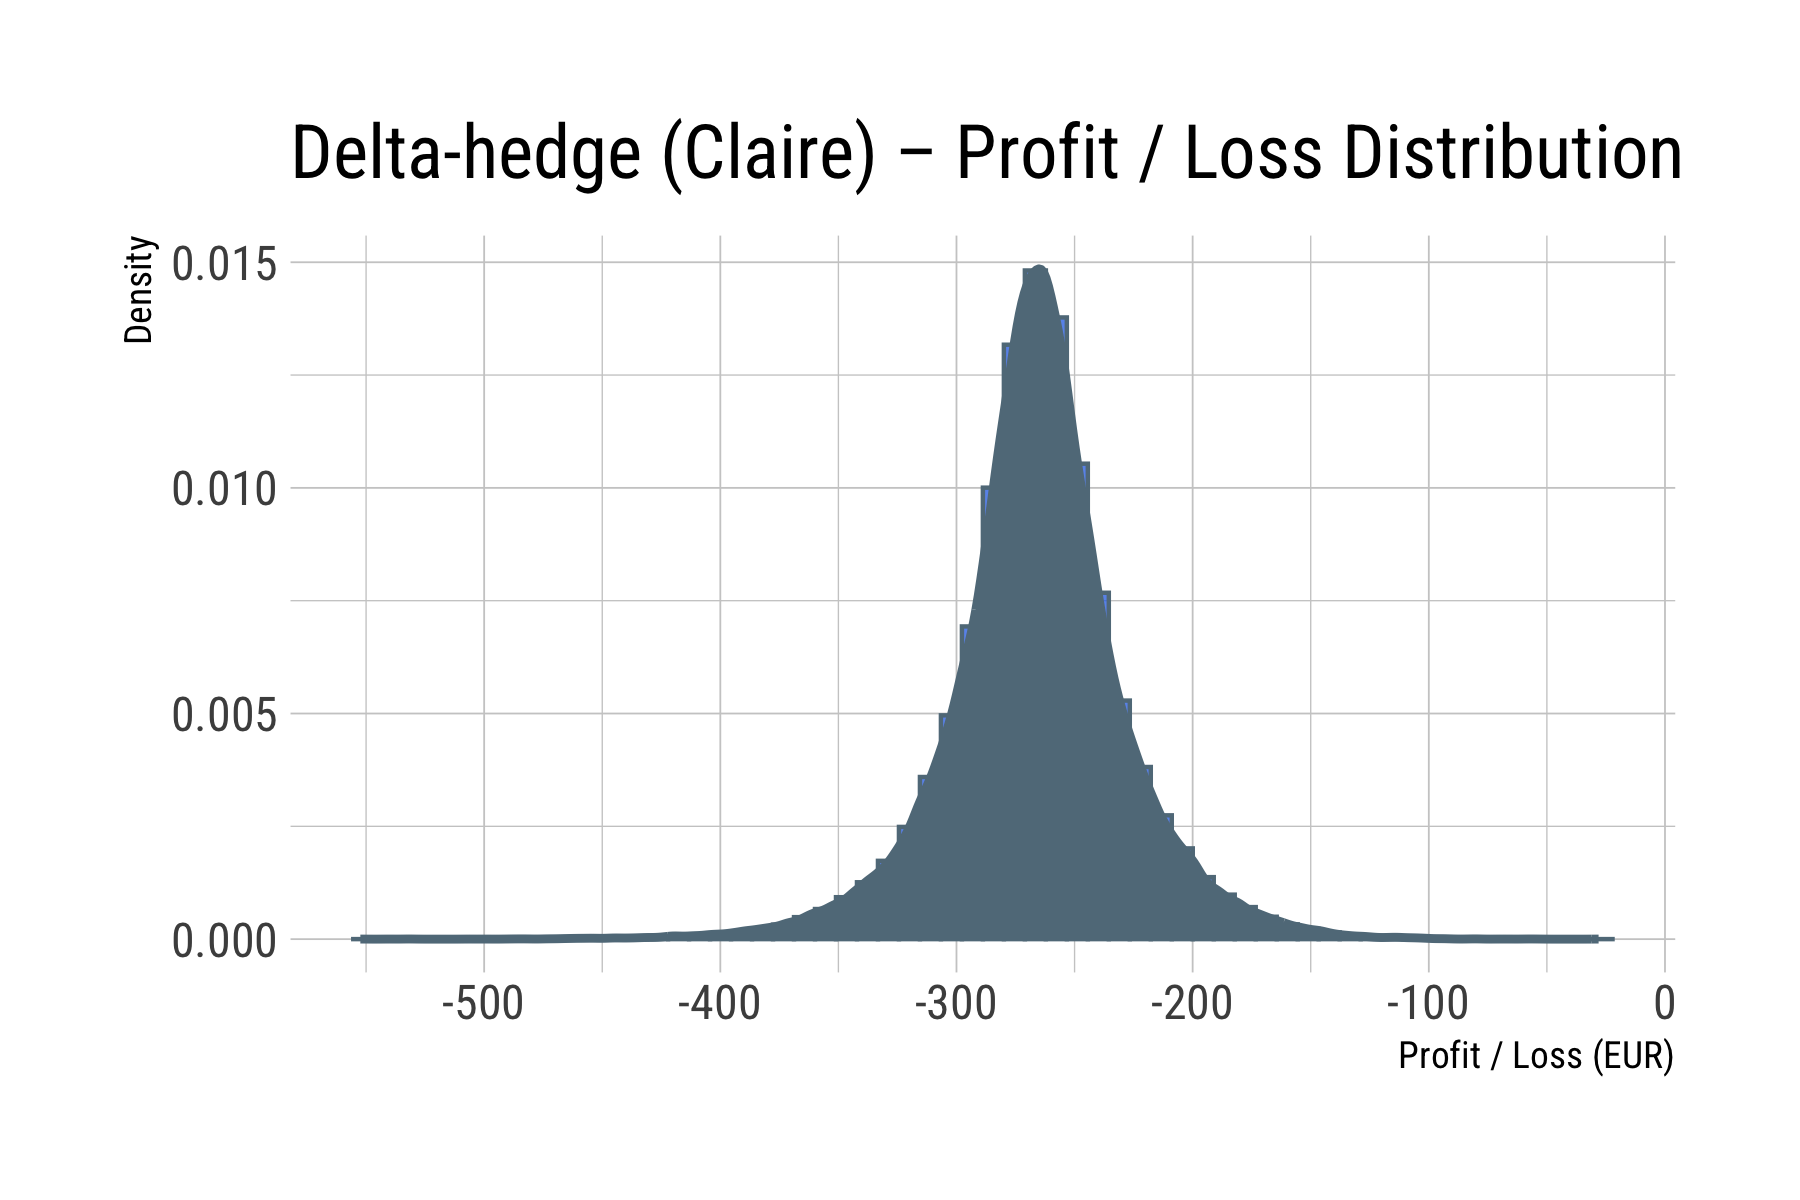
\includegraphics[width=0.85\linewidth]{figures/pnl_claire.png}
	\caption{Profit/Loss distribution — Delta-hedging (Claire)}
	\label{fig:pnl_claire}
\end{figure}

For Claire and the delta hedge strategy, we have the ``best'' distribution. Her exposure throughout the option is kept near zero, so the distribution is centered just above the break-even price with an almost symmetrical spread (skewness and kurtosis are close to a normal curve). Claire pays a ``running cost'' in fees (the residual spread of \(\approx \pm€50\)) to cover her risk and avoid the loss tail that affects Alice and Bradley.

From these histograms, we clearly see that Alice’s strategy (no hedge) is cheap but very risky. Hedging with stop-loss reduces Bradley’s expected losses, but an oscillation can still cause problems, while Claire’s proactive delta hedging strategy almost eliminates the downside risk but demands very tight discipline. The trade-offs are quantified in the rest of the report in terms of both utility and euros.

\begin{figure}[H]
	\centering
	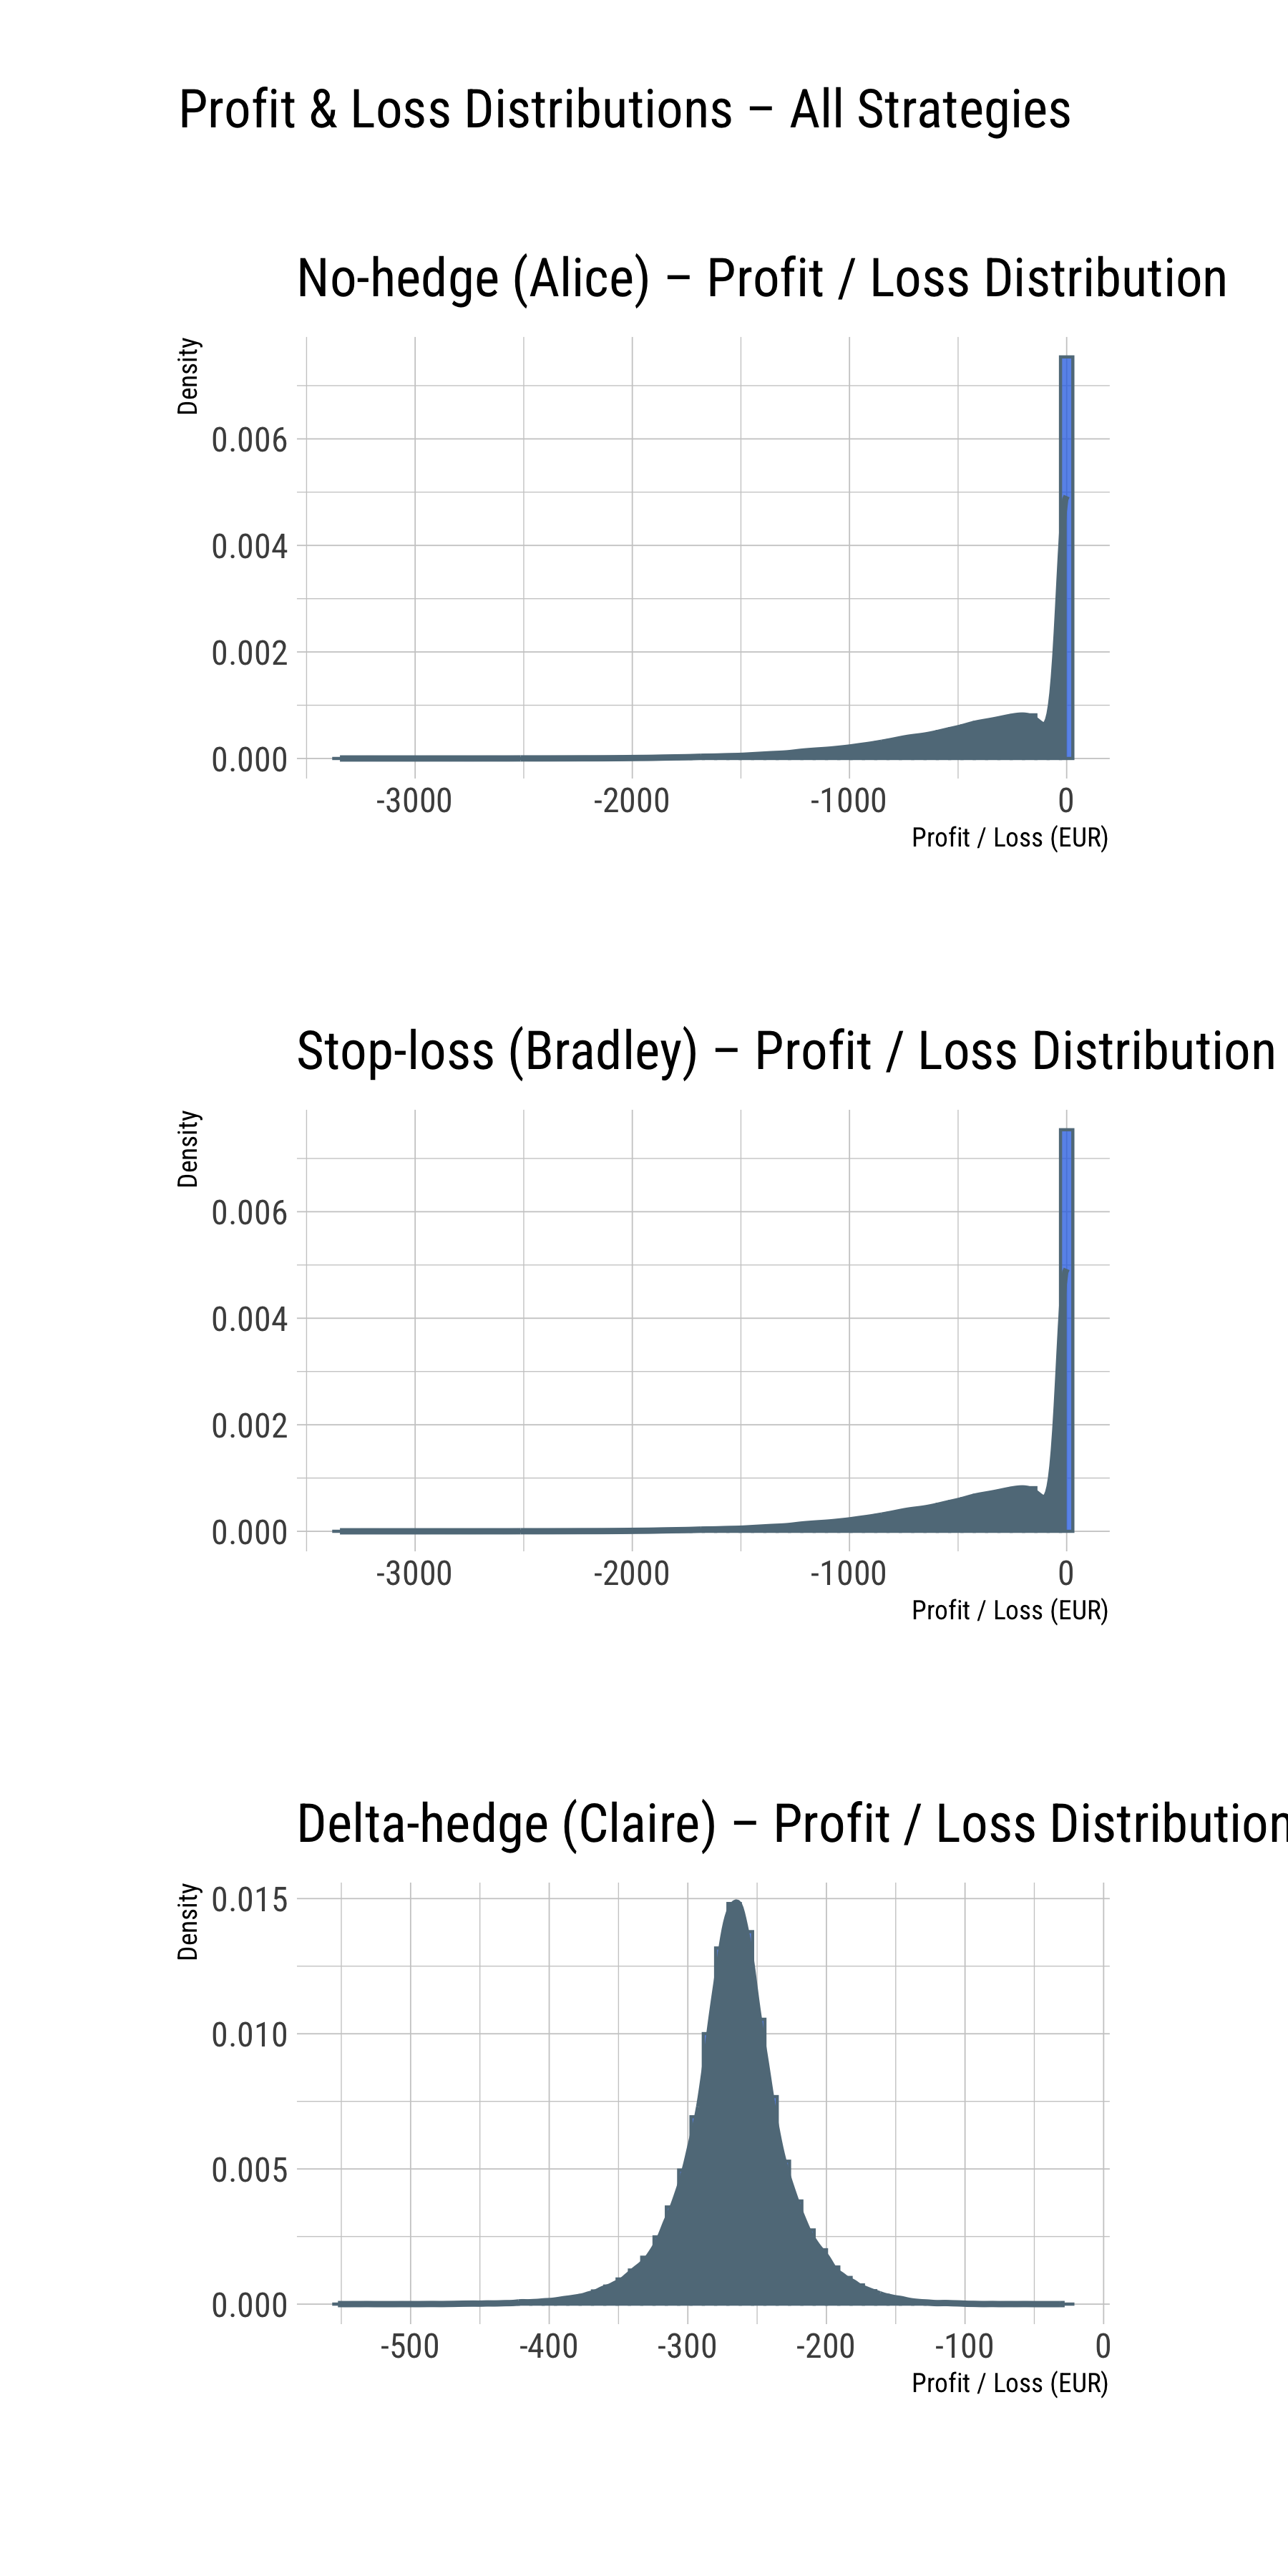
\includegraphics[width=0.5\linewidth]{figures/pnl_all_strategies.png}
	\label{fig:pnl_all_strategies}
\end{figure}
	\subsection{Indifference Prices}
	Discuss \cref{tab:indiff}.
	
	\begin{table}[H]
		\centering
		\caption{Indifference price $P_0^*$ for different risk aversions}
		\label{tab:indiff}
		% TODO: Insert auto‑generated table from R
		\begin{tabular}{@{}lc@{}}
			\toprule
			$a$ & $P_0^*$ (\EUR{}) \\
			\midrule
			1 & 3200 \\
			5 & 2800 \\
			10 & 2500 \\
			\bottomrule
		\end{tabular}
	\end{table}
	
	\subsection{Down‑and‑Out Conditional Probability}
	Present value $\hat p_{\text{DO}|\text{ITM}}=0.12$ and interpret.
	
	% =============================================================
	\section{Discussion}
	% TODO: Compare strategies on risk, complexity, capital efficiency, etc.
	
	% =============================================================
	\section{Conclusion}
	% TODO: Key takeaways, managerial implications, future work.
	
	% =============================================================
	\appendix
	\section{Appendix A}
\begin{lstlisting}[language=R, caption={R code used for generating Figures 1,2,3, and 4}]
	############################################
	
	# ----- libraries -----
	library(ggplot2)
	library(hrbrthemes)   # supplies theme_ipsum_rc()
	# If you want the three-in-one layout later, load patchwork:
	library(patchwork)
	
	# ----- helper: histogram of a single strategy -----
	plot_pnl_hist <- function(pnl_vec,
	strategy_name,
	bins = 60,
	file_out = NULL,
	width = 6,
	height = 4) {
		
		g <- ggplot(data.frame(pnl = pnl_vec),
		aes(x = pnl)) +
		geom_histogram(aes(y = after_stat(density)),
		bins  = bins,
		fill  = "#2b70e4",
		alpha = 0.75) +
		geom_density(size = 1) +
		labs(title = paste0(strategy_name,
		" - Profit / Loss Distribution"),
		x      = "Profit / Loss (EUR)",
		y      = "Density") +
		theme_ipsum_rc()
		
		if (!is.null(file_out)) {
			ggsave(file_out, g,
			width = width, height = height, dpi = 300)
		}
		
		return(invisible(g))
	}
	
	# ----- generate and (optionally) save individual plots -----
	p_A <- plot_pnl_hist(P_and_L, "No-hedge (Alice)",
	file_out = "pnl_alice.png")
	
	p_B <- plot_pnl_hist(P_and_L_B, "Stop-loss (Bradley)",
	file_out = "pnl_bradley.png")
	
	p_C <- plot_pnl_hist(P_and_L_C, "Delta-hedge (Claire)",
	file_out = "pnl_claire.png")
	
	library(patchwork)
	combined <- (p_A / p_B / p_C) + plot_annotation(
	title = "Profit & Loss Distributions - All Strategies",
	theme = theme_ipsum_rc())
	ggsave("pnl_all_strategies.png",
	combined, width = 6, height = 12, dpi = 300)
	
	if (exists("path_df")) {
		g_path <- ggplot(path_df, aes(x = day, y = price)) +
		geom_line(size = 0.7) +
		labs(title = "Example Simulated Stock Path",
		x = "Trading Day", y = "Price (EUR)") +
		theme_ipsum_rc()
		ggsave("sample_path.png", g_path, width = 6, height = 4, dpi = 300)
	}
\end{lstlisting}

	
\end{document}